\chapter{温度や湿度、明るさを測ってみよう}
\section{ファイルとディレクトリ}
\subsection{ファイル、ディレクトリってなんだろう?}
ファイルはコンピュータに保存されている文章、画像、音楽などのデータです。
多くの場合、人間はコンピュータにファイルを操作させることで仕事をします。
ファイルには「\ruby{拡張子}{かく|ちょう|し}」がついており、
そのファイルがどんな種類なのかを表します。
たとえば、画像ファイルを表す.jpgや、動画ファイルを表す.mp4、
テキストファイルを表す.txtなどがあります。

\begin{table}[H]
  \begin{center}
    \caption[tab:files]{ファイルの種類}
    \begin{tabular}{|c|c|c|} \hline
    \begin{minipage}{0.3\hsize}
      \begin{center}
        
\includegraphics[width=\linewidth]{images/chap03/text03-img001.png}
      \end{center}  
    \end{minipage} & 
    \begin{minipage}{0.3\hsize}
      \begin{center}
        
\includegraphics[width=\linewidth]{images/chap03/text03-img002.png}
      \end{center}
    \end{minipage} &
    \begin{minipage}{0.3\hsize}
      \begin{center}
        
\includegraphics[width=\linewidth]{images/chap03/text03-img003.png}
      \end{center} 
    \end{minipage} \\ \hline
    oto.mp3 & gazou.jpg & douga.mp4 \\ \hline
  \end{tabular}
 \end{center}
\end{table}


ディレクトリはファイルをまとめたものです。
ファイルを紙だとしてディレクトリはバインダーだと思うとわかりやすいでしょう。
1回目で習ったフォルダと同じものです。今回はディレクトリという名前を使います。

\begin{tcolorbox}[title=\useOmetoi]
\begin{enumerate}
\item ファイルとはなんでしょうか。\\
\underline{答え.\hspace{0.8\linewidth}}
\item ディレクトリとはなんでしょうか。\\
\underline{答え.\hspace{0.8\linewidth}}
\item どんな拡張子があるかインターネットで調べてみましょう。
\end{enumerate}

\begin{table}[H]
  \centering
  \begin{tabular}{lrr} \toprule
番号 & 拡張子 & 表すもの \\ \midrule
1. & .jpg & 画像 \\
2. & .mp4 & 動画 \\
3. & \hspace{10\zw} & \hspace{10\zw} \\
4. & \hspace{10\zw} & \hspace{10\zw} \\
5. & \hspace{10\zw} & \hspace{10\zw} \\ \bottomrule
\end{tabular}
\end{table}
例を見て、拡張子とその拡張子が何を表すか2つ書いてみましょう。
\end{tcolorbox}

\subsection{ディレクトリの関係}
いまのディレクトリの中に入っているディレクトリを\emph{下のディレクトリ}、
いまのディレクトリを中に持っているディレクトリを\emph{上のディレクトリ}と呼びます。

一番上のディレクトリは / スラッシュで書きます。その下にあるbin boot dev etcなどのディレクトリはコンピュータの設定ファイルを持っているので、間違った使い方をすると壊れます。気を付けましょう。

ユーザが作業に使ってもよいディレクトリを\emph{ホームディレクトリ}と言います。
ユーザの作業はホームディレクトリの下で行います。
ホームディレクトリは、ラズベリーパイでは\emph{/home/pi}です。
みなさんが今、作業に使っているディレクトリは\emph{カレントディレクトリ}と言います。
カレントディレクトリは./と書くことができます。
カレントディレクトリから一つ上のディレクトリは../と書くことができます。
ディレクトリは/で区切ります。

ディレクトリの位置は\emph{一番上のディレクトリ(/)から見てどこにあるか(絶対パス)}、または\emph{カレントディレクトリから見てどこにあるか(相対パス)}で決まります。

絶対パスの特徴は\emph{パスの先頭に / をつけます}。相対パスの特徴は\emph{パスの先頭に / をつけません}。

ディレクトリがxxxのとき xxxまたは xxx/と書きます。ディレクトリがxxxのとき xxxまたは./xxxと書きます。

図\ref{fig:folder-path}にフォルダとフォルダの関係をパスであらわしてあります。パスとフォルダ間の関係を考えながら図を読みましょう。

\begin{figure}[H]
    \begin{minipage}{0.4\hsize}
        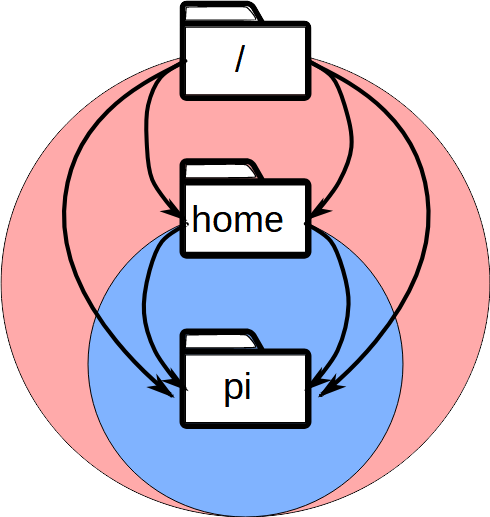
\includegraphics[width=\hsize]{images/chap03/text03-img004.png}
    \end{minipage}
    \begin{minipage}{0.6\hsize}
        \begin{itemize}
        \item /は一番上のディレクトリから見ると/
        \item /はカレントディレクトリが/のとき./
        \item /はカレントディレクトリがhomeのとき../
        \item /はカレントディレクトリがpiのとき../../
        \item homeは一番上のディレクトリから見ると/home
        \item homeはカレントディレクトリが/のとき./home
        \item homeはカレントディレクトリがhomeのとき./
        \item homeはカレントディレクトリがpiのとき../
        \item piは一番上のディレクトリから見ると/home/pi
        \item piはカレントディレクトリが/のとき./home/pi
        \item piはカレントディレクトリがhomeのとき./pi
        \item piはカレントディレクトリがpiのとき./
        \end{itemize}
    \end{minipage}
    \caption{フォルダ間の関係をパスで説明する}
    \label{fig:folder-path}
\end{figure}

\begin{tcolorbox}[title=\useOmetoi]
\begin{figure}[H]
 \centering
 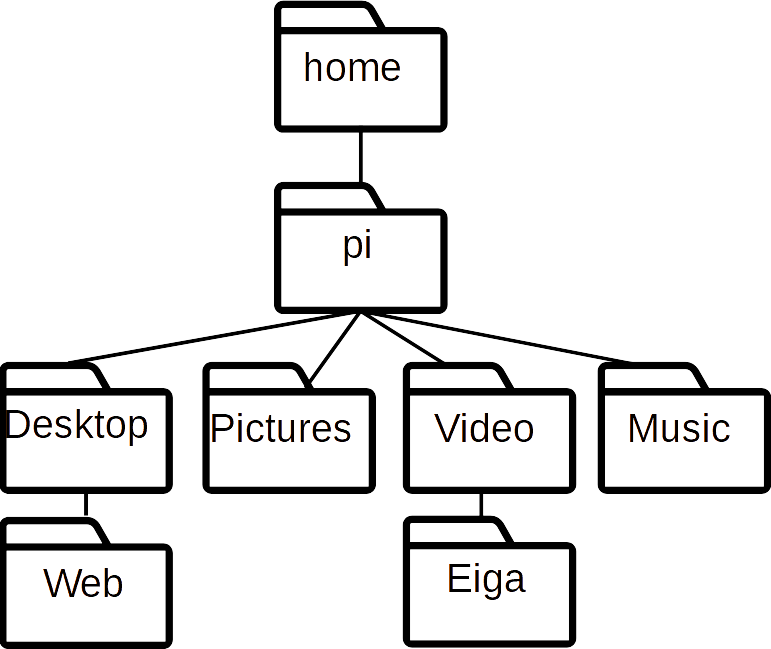
\includegraphics[width=0.6\linewidth]{images/chap03/text03-img005.png}
\end{figure}
\begin{enumerate}
\item ホームディレクトリはどれでしょうか\\
\underline{答え.\hspace{0.8\linewidth}}
\item カレントディレクトリが/home/pi/Videoのとき、上のディレクトリはどれでしょうか。\\
\underline{答え.\hspace{0.8\linewidth}}
\item カレントディレクトリが/home/piのとき、下のディレクトリはどれでしょうか。4つあります。\\
\underline{答え.\hspace{0.8\linewidth}}
\item カレントディレクトリが/home/pi/Desktopのとき、上のディレクトリはどれでしょうか。\\
\underline{答え.\hspace{0.8\linewidth}}
\item カレントディレクトリが/home/pi/Desktopのとき、下のディレクトリはどれでしょうか。\\
\underline{答え.\hspace{0.8\linewidth}}
\end{enumerate}
\end{tcolorbox}
